
\captionsetup{justification=centering, labelfont=bf}


\subsection{Non-Ideal Op-Amp}
\begin{figure}[H]
    \centering
    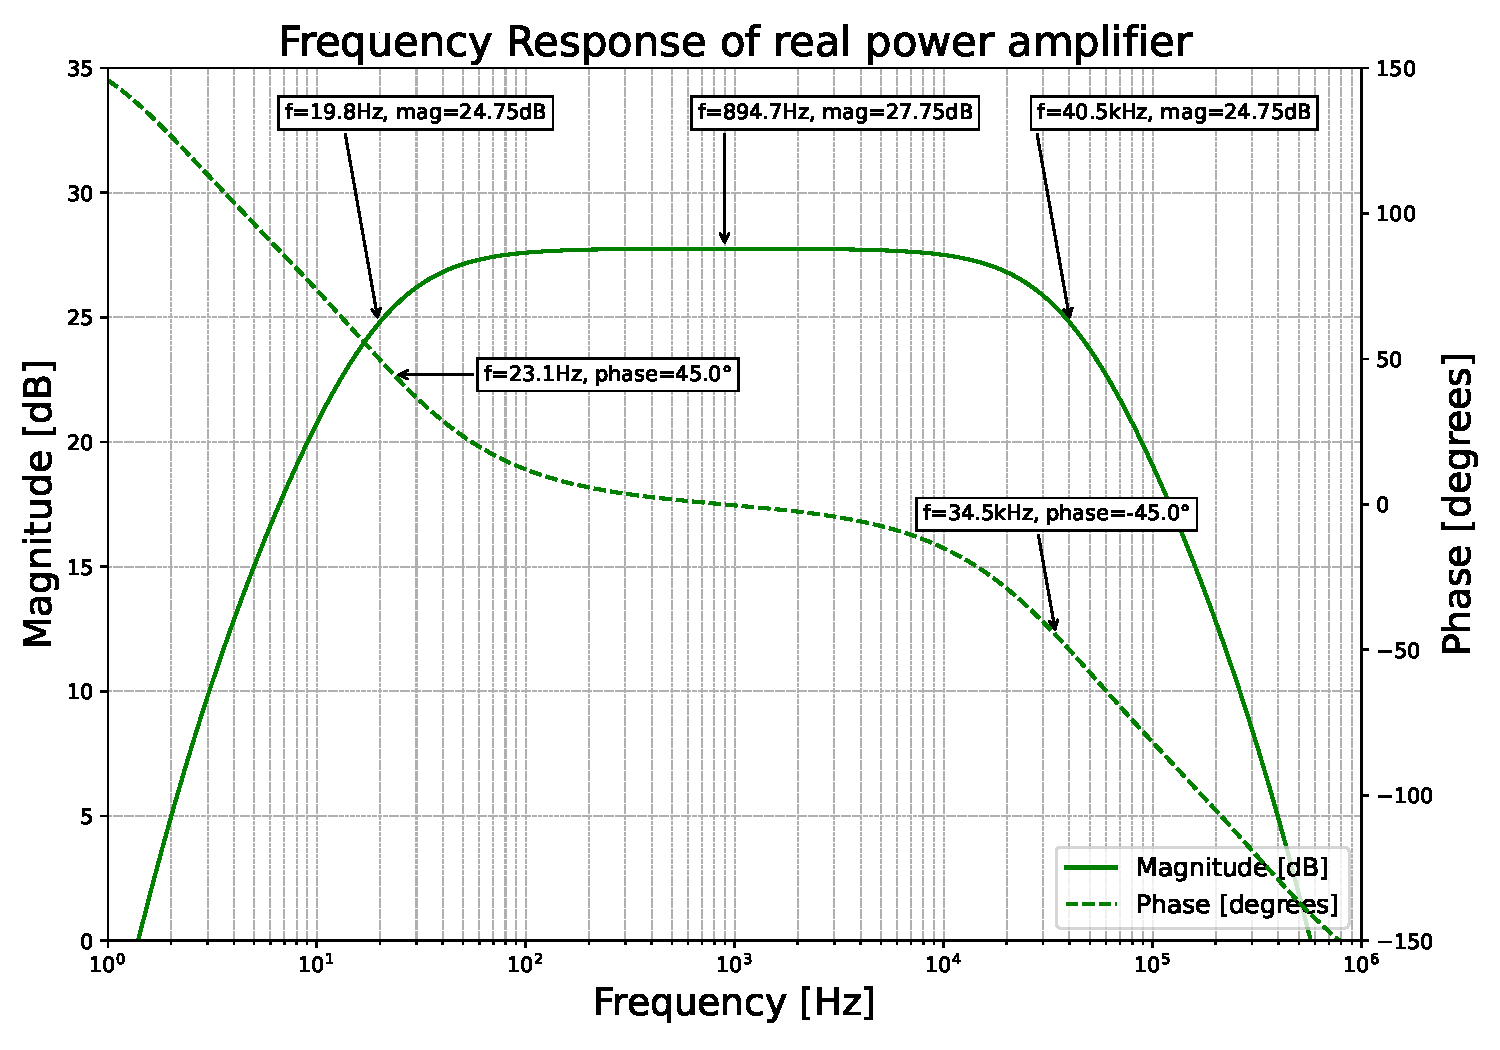
\includegraphics[width=0.9\linewidth]{TU Delft Booming Bass Project Report/figures/PowerAmplifier/not ideal amplifier results.pdf}
    \captionsetup{justification=raggedright, labelfont=bf}
    \caption{The results of the power amplifier circuit, using what were considered to be the ideal component values, are shown.}
    \label{fig:not ideal amplifier}
\end{figure}
\newpage
\subsection{Calculation of $\mathbf{R_c}$}
\label{calculation of Rc}
The circuit diagram used to calculate $R_c$ is shown in Fig. \ref{fig: non ideal active high}:

\begin{figure}[H]
    \centering
    \begin{minipage}[T]{0.55\textwidth}
        \centering
        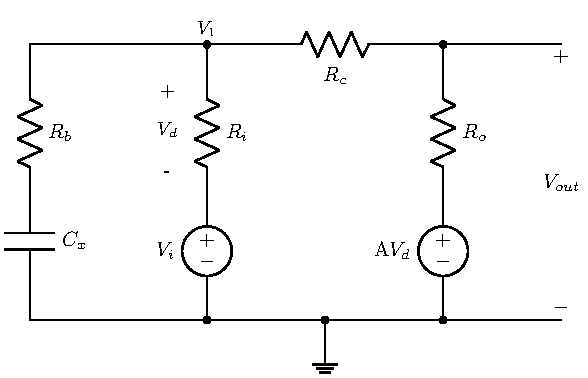
\includegraphics[width=\linewidth]{TU Delft Booming Bass Project Report/figures/PowerAmplifier/circuits/non_ideal opamp circuit.pdf}
        \captionsetup{justification=raggedright, labelfont=bf}
        \caption{The non-ideal equivalent circuit to \autoref{fig: pa active high pass}.}
        \label{fig: non ideal active high}
    \end{minipage}%
    \hspace{0.05\textwidth} % Adjust space between figure and table
    \begin{minipage}[T]{0.35\textwidth}
        \centering
        \begin{tabular*}{0.9\textwidth}{@{\extracolsep{\fill}} c c @{}}
            \toprule
            \textbf{Component} & \textbf{Value of Component} \\
            \midrule
            \textbf{$C_x$} & 79.5$\mu$F \\
            \textbf{$R_b$} & 1k$\Omega$ \\ 
            \textbf{$R_i$} & 200k$\Omega$ \\
            \textbf{$R_o$} & 10$\Omega$ \\
            A & $10^5$ \\
            \bottomrule
        \end{tabular*}
        \captionsetup{justification=raggedright, labelfont=bf}
        \caption{Component values in the non-ideal circuit.}
        \label{tab:ideal values}
    \end{minipage}
\end{figure}







From the circuit, it is clear that the following holds:
\begin{flalign*}
    V_o = 25V_i, \quad V_d = V_1 - V_i
\end{flalign*}
Applying nodal analysis at node $V_1$ in circuit of Fig. \ref{fig: non ideal active high}, gives:
\begin{flalign*}
    \frac{V_{o}-V_{1}}{R_C} + \frac{V_o- 10^5(V_1-V_i)}{R_o} =0 \\
    10(25V_i - V_1) + R_c\left(25V_i - 10^5(V_1 - V_i)\right) = 0 \\
     R_c = -\frac{10(25V_i-V_1)}{25V_i - 10^5V_1 + 10^5V_i} \\
\end{flalign*}

\begin{flalign}
    25V_i + 10^5V_i \approx 10^5 V_i
\end{flalign}

\begin{flalign}
\label{eq: 1}
    R_c = -\frac{25 V_i - V_1}{10^4(V_i-V_1)}
    \equnit{\si{\Omega}}
\end{flalign}


Applying nodal analysis at node 2 gives:
\[\frac{V_1}{R_b + Z_c} + \frac{V_1-V_i}{R_i} + \frac{V_1-V_o}{Rc} = 0\]
\[\frac{V_1 R_c}{R_b + Z_c} + \frac{(V_1-V_i)R_c}{R_i} + {V_1-V_o} = 0\]

\[R_c\left(\frac{V_1}{R_b + Z_c} + \frac{V_1-V_i}{R_i}\right) =  25V_i-V_1\]

\begin{equation}
\label{eq: 2}
    Rc = \frac{25V_i-V_1}{\frac{V_1}{R_b + Z_c} + \frac{V_1-V_i}{R_i}}
\end{equation}

By comparing Eq. (\ref{eq: 1}) and (\ref{eq: 2}), follows that:
\[ -\frac{25 V_i - V_1}{10^4V_i - 10^4 V_1} = \frac{25V_i-V_1}{\frac{V_1}{R_b + Z_c} + \frac{V_1-V_i}{R_i}}\]
\[10^4(V_1-V_i) = \frac{V_1}{R_b + Z_c} + \frac{V_1-V_i}{R_i}\]

\[\left(\frac{1}{R_b + Z_c} + \frac{1}{R_i}-10^4\right)V_1 = \left(\frac{1}{R_i}-10^4\right)V_i\] 
For $R_i=200\text{k}\Omega$, gives: 
\[\frac{1}{R_i} -10^4 \Rightarrow \frac{1}{200k} - 10^4 \approx -10^4\]
\begin{flalign}
\label{eq: 3}
    V_1 = \left(\frac{-10^4}{\frac{1}{R_b + Z_c}-10^4}\right)Vi = aV_i
\end{flalign}
where $a = 1-7.95\cdot10^{-16} j\omega$. Substituting Eq. (\ref{eq: 3}) in (\ref{eq: 1}), gives that:
\begin{flalign*}
    R_c = \frac{a-25}{10^4(a-1)}\left(\frac{V_i}{V_i}\right)
    \equnit{\si{\Omega}}
\end{flalign*}

Putting these values in a calculator gives that $R_c$:
\begin{flalign*}
    R_c= (2.4\cdot10^{4}) - 1.9j\omega\cdot10^{-3}\Omega
    \equnit{\si{\Omega}}
\end{flalign*}

The real part is approximately an order of 7 greater than the imaginary part, making the imaginary component negligible until frequencies well beyond the circuit's requirements and operation conditions, resulting in:
\begin{flalign*}
    R_c \approx 24k\Omega \Rightarrow R_c= 24R_b
\end{flalign*}







\subsection{Total Transfer Function Derivation}
\label{total transfer}

To obtain the total transfer function, the functions \ref{eq: E}, \ref{eq: F} and \ref{eq: G} must be multiplied together. This can be done as follows:


\begin{flalign*}
    \mathbf{E(\omega)} = \frac{R_2 C_1 s}{s R_1 C_1 + 1}, \quad \mathbf{F(\omega)} = \frac{1}{s R_a C_a + 1}, \quad \mathbf{G(\omega)} = \frac{R_C}{R_b + \frac{1}{s C_x}}+1
\end{flalign*}

Let $a = R_2 C_1$, $b = R_a C_a$, $d =ab$, $f = R_b C_x$, and $k = R_2 C_1 R_c C_x$:
\begin{flalign*}
    \frac{sa}{s a + 1}\left(\frac{1}{s b + 1}\right) = \frac{sa }{(s a + 1)(s b + 1)}
\end{flalign*}
\begin{flalign*}
    \mathbf{H(\omega)} = \frac{sa}{s^2 d + s a + s b + 1}=\frac{sa}{e}
\end{flalign*}
where $e = s^2 d + s a + s b  + 1$, gives:
\begin{flalign*}
    \frac{sa }{e}\left(\frac{R_C}{R_b + \frac{1}{s C_x}}+1 \right) = \frac{sa }{e}\left( \frac{s R_C C_x}{s R_b C_x  + 1}+1 \right)
\end{flalign*}






\[
\frac{s a}{e} + \frac{s^2 k}{e(sR_b C_x+1)} = \frac{s a (sf + 1) + s^2 k}{e \big(sf + 1 \big)}
\]

\[\frac{s^2( af+ k) + s a }{e \big(sf + 1 \big)}\]

Substituting all of the variables given earlier, gives:
\begin{flalign*}
    \mathbf{H(\omega)} = \frac{s^2 R_2 C_1 R_b C_x + s^2 R_2 C_1 R_c C_x+ s R_2 C_1 }{(s^2 C_1 C_a R_2 R_a + sC_a R_a + sC_1 R_2+1)(R_b C_x s + 1 )}
\end{flalign*}
\begin{flalign}\label{eq: third order}
    e(sf+1) &= (s^2 d+ s(a+b) +1)(sf + 1 ) \notag\\
            &= s^3df + s^2f(a+b) +sf + s^2d + s(a+b) + 1 \notag\\
            &= s^3df + s^2(f(a+b) + d) + s(a+b+f) + 1
\end{flalign}

Thus giving:
\begin{flalign*}
    \mathbf{H(\omega)} = \frac{s^2( af+ k) + s a }{s^3df + s^2(f(a+b) + d) + s(a+b+f) + 1}
\end{flalign*}
Let $t = a+b+f$, $q = af + k$, and $r = f(a+b) + d$:

%( \[\frac{\frac{1}{s^2}}{\frac{1}{s^2}} \cdot H(\omega) = \frac{R_2 C_1 R_b C_x + R_c R_2 C_1 C_x+  \frac{R_2 C_1}{s} }{sdf + f(a+b) + d + \frac{1}{s}(a+b+f) + \frac{1}{s^2}}\])\\
This gives: 
\begin{flalign}
\mathbf{H(\omega)} &= \frac{s^2q+ s a }{ (s^2r + 1) + s(s^2df + t)}
\end{flalign}
\subsubsection{Derivation for Phase Formula}
\label{sec: phase calc}
To calculate the phase, $\mathbf{H(\omega)}$ must be multiplied by its complex conjugate. After separating the real and imaginary parts of the enumerator, the expression becomes:
\begin{flalign*}
    \mathbf{H(\omega)} &= \frac{s^2q+ s a }{ (s^2r + 1) + s(s^2df + t)}\left(\frac{(s^2r + 1) - s(s^2df + t)}{(s^2r + 1) - s(s^2df + t)}\right)\\
                        &= \frac{(s^2q + s a)((s^2r + 1) - s(s^2df + t)) }{ (s^2r + 1)^2 - s^2(s^2df + t)^2}
\end{flalign*}
\begin{flalign*}
    h = (s^2r + 1)^2 - s^2(s^2df + t)^2
\end{flalign*}

Multiplying the denominator by the first part of the conjugate results in:
\begin{flalign*}
    &= (s^2q+ s a)(s^2r + 1) \\
    &=s^4qr +  s^3ar +s^2q + sa
\end{flalign*}
And thus giving for its real and imaginary part:
\begin{flalign*}
    \text{Re}_1= \frac{\omega^4qr - \omega^2q}{h} \\
    \text{Im}_1 = \frac{\omega a-\omega^3ar}{h}
\end{flalign*}

Multiplying the denominator by the second part of the conjugate results in:
\begin{flalign*}
    (s^2q+ s a)(-s(s^2df + t) ) &= -s(s^2q+ s a)(s^2df + t ) \\
                                &=-s^5dfq - s^3qt - s^2at - s^4adf
\end{flalign*}

Thus resulting in: 
\begin{flalign*}
    \text{Re}_2 = \frac{\omega^2at-\omega^4adf}{h} \\
    \text{Im}_2 = \frac{\omega^3qt-\omega^5dfq}{h}
\end{flalign*}

For the total real and imaginary part, the following holds:
\begin{flalign*}
    \text{Re} = \text{Re}_1 + \text{Re}_2 \notag\\
    \text{Im} = \text{Im}_1 + \text{Im}_2 \notag\\
    \phi_{\text{Phase}} = \arctan\left(\frac{\text{Im}}{\text{Re}}\right)
\end{flalign*}







\newpage




\DeclareTCBListing{mintedbox}{O{}m!O{}}{%
  breakable=true,
  listing engine=minted,
  listing only,
  minted language=#2,
  minted style=default,
  minted options={%
    linenos,
    gobble=0,
    breaklines=true,
    breakafter=,,
    fontsize=\small,
    numbersep=8pt,
    #1},
  boxsep=0pt,
  left skip=0pt,
  right skip=0pt,
  left=25pt,
  right=0pt,
  top=3pt,
  bottom=3pt,
  arc=5pt,
  leftrule=0pt,
  rightrule=0pt,
  bottomrule=2pt,
  toprule=2pt,
  colback=bg,
  colframe=orange!70,
  enhanced,
  overlay={%
    \begin{tcbclipinterior}[h!]
    \fill[orange!20!white] (frame.south west) rectangle ([xshift=20pt]frame.north west);
    \end{tcbclipinterior}},
  #3}
